\section{Primera captura: Laboratorio de Pabellón 1}

\par Para una primera experimentación, decidimos correr la herramienta sniffer en la red interna del pabellón 1 de Ciudad Universitaria. Nos conectamos por Wifi a la red y tomamos muestras durante 17 minutos. Utilizamos la fuente de información S1 para diferenciar cada host como un símbolo. Luego, calculamos la información de cada host y con esto, la entropía de la fuente (red).

\par En el gráfico \ref{fig:exp1_labo_infovsentro} se pueden ver los 25 hosts con menor información. La linea punteada roja representa la entropía de la fuente y, como se observa rápidamente, hay un solo host que se encuentra del lado izquierdo (\textbf{10.210.210.199}). Esto significa que es un símbolo con muy poca información y por ende, mucha probabilidad. Para nosotros, esto significa que es un host que participa mucho de la red, preguntando constantemente qué dirección MAC corresponde a una dirección IP. Tomamos entonces a este host como un nodo distinguido de la red.

\begin{figure}[h]
  \begin{subfigure}[b]{.5\textwidth}
    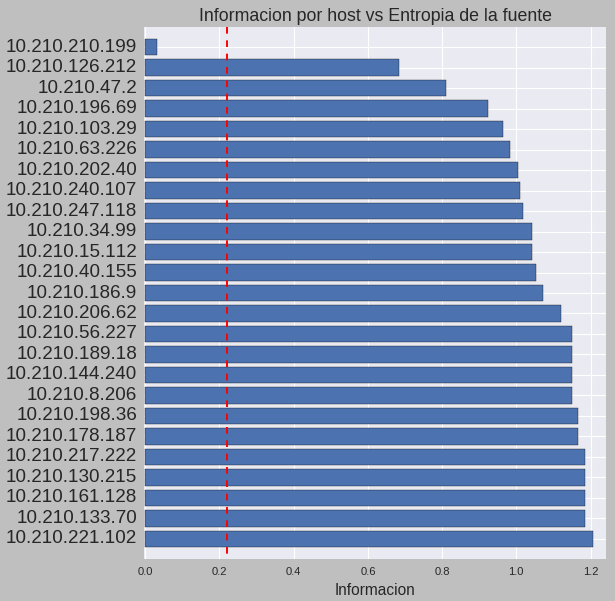
\includegraphics[width=\textwidth]{imagenes/laboratorio/informaciones_vs_entropia.png}
  \end{subfigure}
  \label{fig:exp1_labo_infovsentro}
  \caption{Información de cada símbolo (host) de la red comparada con el valor de la entropía de la fuente de información (red local). Se limita el gráfico a los 25 símbolos con menor valor de información.}
\end{figure}

\par La distinción del host con IP \textbf{10.210.210.199} la podemos corroborar en el gráfico de la figura \ref{fig:exp1_labo_grafo}. Este grafo representa a la red relacionando nodos con hosts y aristas con mensajes. El diámetro de los nodos está dado por el nivel de participación que tiene en las capturas tomada. Este valor fue calculado teniendo en cuenta los siguientes parámetros:
\begin{itemize}
	\item Cantidad de mensajes ARP enviados (solo tomando los del tipo who-has).
	\item Cantidad de mensajes ARP que consultaban por su ip (solo tomando los del tipo who-has).
	\item Cantidad de hosts \textit{distintos} por los cuales preguntó su dirección MAC.
	\item Cantidad de hosts \textit{distintos} que preguntaron por mi dirección MAC.
\end{itemize}
\par Las aristas por su parte, representan la consulta de un host por la dirección MAC de otro (sin diferenciar la dirección de los mensajes). Y el peso de cada arista (expresado como grosor) está dado por la cantidad de mensajes que relacionan los hosts.

\begin{figure*}[ht]
  \hspace*{-0.5cm}
  \begin{subfigure}[b]{1.1\textwidth}
    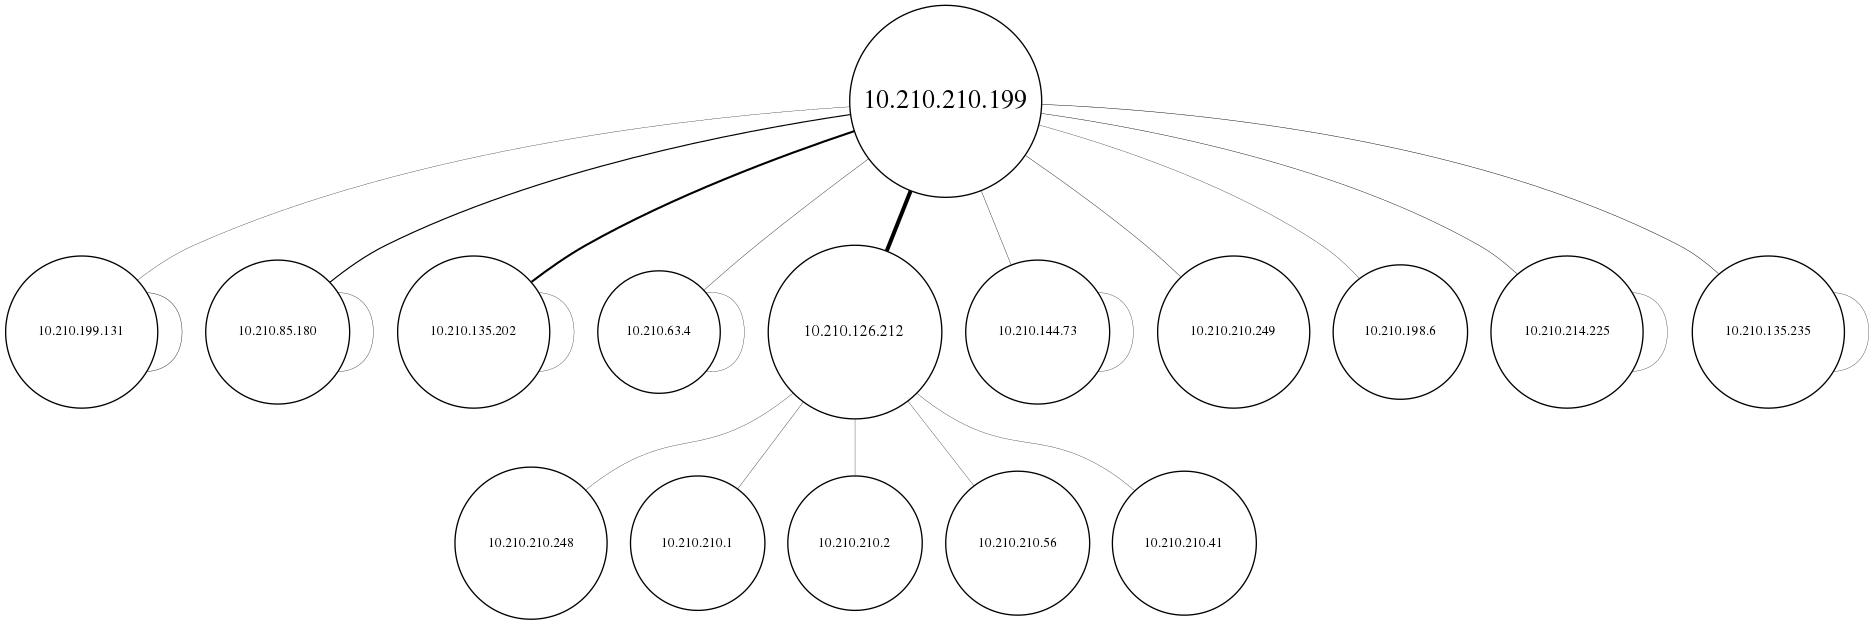
\includegraphics[width=\textwidth]{imagenes/laboratorio/grafo_10.png}
  \end{subfigure}
	\label{fig:exp1_labo_grafo}
	\caption{Grafo con los nodos mas interesantes de la red de la primer captura. El diámetro del nodo implica mayor participación.}
\end{figure*}
